\documentclass[twoside]{book}

% Packages required by doxygen
\usepackage{fixltx2e}
\usepackage{calc}
\usepackage{doxygen}
\usepackage[export]{adjustbox} % also loads graphicx
\usepackage{graphicx}
\usepackage[utf8]{inputenc}
\usepackage{makeidx}
\usepackage{multicol}
\usepackage{multirow}
\PassOptionsToPackage{warn}{textcomp}
\usepackage{textcomp}
\usepackage[nointegrals]{wasysym}
\usepackage[table]{xcolor}

% Font selection
\usepackage[T1]{fontenc}
\usepackage[scaled=.90]{helvet}
\usepackage{courier}
\usepackage{amssymb}
\usepackage{sectsty}
\renewcommand{\familydefault}{\sfdefault}
\allsectionsfont{%
  \fontseries{bc}\selectfont%
  \color{darkgray}%
}
\renewcommand{\DoxyLabelFont}{%
  \fontseries{bc}\selectfont%
  \color{darkgray}%
}
\newcommand{\+}{\discretionary{\mbox{\scriptsize$\hookleftarrow$}}{}{}}

% Page & text layout
\usepackage{geometry}
\geometry{%
  a4paper,%
  top=2.5cm,%
  bottom=2.5cm,%
  left=2.5cm,%
  right=2.5cm%
}
\tolerance=750
\hfuzz=15pt
\hbadness=750
\setlength{\emergencystretch}{15pt}
\setlength{\parindent}{0cm}
\setlength{\parskip}{3ex plus 2ex minus 2ex}
\makeatletter
\renewcommand{\paragraph}{%
  \@startsection{paragraph}{4}{0ex}{-1.0ex}{1.0ex}{%
    \normalfont\normalsize\bfseries\SS@parafont%
  }%
}
\renewcommand{\subparagraph}{%
  \@startsection{subparagraph}{5}{0ex}{-1.0ex}{1.0ex}{%
    \normalfont\normalsize\bfseries\SS@subparafont%
  }%
}
\makeatother

% Headers & footers
\usepackage{fancyhdr}
\pagestyle{fancyplain}
\fancyhead[LE]{\fancyplain{}{\bfseries\thepage}}
\fancyhead[CE]{\fancyplain{}{}}
\fancyhead[RE]{\fancyplain{}{\bfseries\leftmark}}
\fancyhead[LO]{\fancyplain{}{\bfseries\rightmark}}
\fancyhead[CO]{\fancyplain{}{}}
\fancyhead[RO]{\fancyplain{}{\bfseries\thepage}}
\fancyfoot[LE]{\fancyplain{}{}}
\fancyfoot[CE]{\fancyplain{}{}}
\fancyfoot[RE]{\fancyplain{}{\bfseries\scriptsize Generated by Doxygen }}
\fancyfoot[LO]{\fancyplain{}{\bfseries\scriptsize Generated by Doxygen }}
\fancyfoot[CO]{\fancyplain{}{}}
\fancyfoot[RO]{\fancyplain{}{}}
\renewcommand{\footrulewidth}{0.4pt}
\renewcommand{\chaptermark}[1]{%
  \markboth{#1}{}%
}
\renewcommand{\sectionmark}[1]{%
  \markright{\thesection\ #1}%
}

% Indices & bibliography
\usepackage{natbib}
\usepackage[titles]{tocloft}
\setcounter{tocdepth}{3}
\setcounter{secnumdepth}{5}
\makeindex

% Hyperlinks (required, but should be loaded last)
\usepackage{ifpdf}
\ifpdf
  \usepackage[pdftex,pagebackref=true]{hyperref}
\else
  \usepackage[ps2pdf,pagebackref=true]{hyperref}
\fi
\hypersetup{%
  colorlinks=true,%
  linkcolor=blue,%
  citecolor=blue,%
  unicode%
}

% Custom commands
\newcommand{\clearemptydoublepage}{%
  \newpage{\pagestyle{empty}\cleardoublepage}%
}

\usepackage{caption}
\captionsetup{labelsep=space,justification=centering,font={bf},singlelinecheck=off,skip=4pt,position=top}

%===== C O N T E N T S =====

\begin{document}

% Titlepage & ToC
\hypersetup{pageanchor=false,
             bookmarksnumbered=true,
             pdfencoding=unicode
            }
\pagenumbering{alph}
\begin{titlepage}
\vspace*{7cm}
\begin{center}%
{\Large B\+M\+E\+D\+E\+MO }\\
\vspace*{1cm}
{\large Generated by Doxygen 1.8.14}\\
\end{center}
\end{titlepage}
\clearemptydoublepage
\pagenumbering{roman}
\tableofcontents
\clearemptydoublepage
\pagenumbering{arabic}
\hypersetup{pageanchor=true}

%--- Begin generated contents ---
\chapter{Hierarchical Index}
\section{Class Hierarchy}
This inheritance list is sorted roughly, but not completely, alphabetically\+:\begin{DoxyCompactList}
\item \contentsline{section}{App\+Delegate()}{\pageref{category_app_delegate_07_08}}{}
\item N\+S\+Object\begin{DoxyCompactList}
\item \contentsline{section}{bmelib}{\pageref{interfacebmelib}}{}
\end{DoxyCompactList}
\item $<$U\+I\+Application\+Delegate$>$\begin{DoxyCompactList}
\item \contentsline{section}{App\+Delegate}{\pageref{interface_app_delegate}}{}
\end{DoxyCompactList}
\item $<$U\+I\+Picker\+View\+Delegate$>$\begin{DoxyCompactList}
\item \contentsline{section}{View\+Controller}{\pageref{interface_view_controller}}{}
\end{DoxyCompactList}
\item U\+I\+Responder\begin{DoxyCompactList}
\item \contentsline{section}{App\+Delegate}{\pageref{interface_app_delegate}}{}
\end{DoxyCompactList}
\item $<$U\+I\+Text\+Field\+Delegate$>$\begin{DoxyCompactList}
\item \contentsline{section}{View\+Controller}{\pageref{interface_view_controller}}{}
\end{DoxyCompactList}
\item U\+I\+View\+Controller\begin{DoxyCompactList}
\item \contentsline{section}{View\+Controller}{\pageref{interface_view_controller}}{}
\end{DoxyCompactList}
\item \contentsline{section}{View\+Controller()}{\pageref{category_view_controller_07_08}}{}
\end{DoxyCompactList}

\chapter{Class Index}
\section{Class List}
Here are the classes, structs, unions and interfaces with brief descriptions\+:\begin{DoxyCompactList}
\item\contentsline{section}{\mbox{\hyperlink{interface_app_delegate}{App\+Delegate}} }{\pageref{interface_app_delegate}}{}
\item\contentsline{section}{\mbox{\hyperlink{category_app_delegate_07_08}{App\+Delegate()}} }{\pageref{category_app_delegate_07_08}}{}
\item\contentsline{section}{\mbox{\hyperlink{interfacebmelib}{bmelib}} }{\pageref{interfacebmelib}}{}
\item\contentsline{section}{\mbox{\hyperlink{interface_view_controller}{View\+Controller}} }{\pageref{interface_view_controller}}{}
\item\contentsline{section}{\mbox{\hyperlink{category_view_controller_07_08}{View\+Controller()}} }{\pageref{category_view_controller_07_08}}{}
\end{DoxyCompactList}

\chapter{Class Documentation}
\hypertarget{interface_app_delegate}{}\section{App\+Delegate Class Reference}
\label{interface_app_delegate}\index{App\+Delegate@{App\+Delegate}}
Inheritance diagram for App\+Delegate\+:\begin{figure}[H]
\begin{center}
\leavevmode
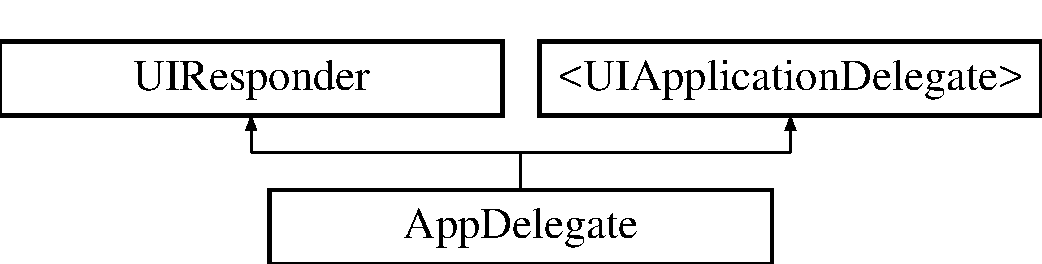
\includegraphics[height=2.000000cm]{interface_app_delegate}
\end{center}
\end{figure}
\subsection*{Instance Methods}
\begin{DoxyCompactItemize}
\item 
\mbox{\Hypertarget{interface_app_delegate_affcb482ed45b506b0659be7277e805f9}\label{interface_app_delegate_affcb482ed45b506b0659be7277e805f9}} 
(void) -\/ {\bfseries save\+Context}
\end{DoxyCompactItemize}
\subsection*{Properties}
\begin{DoxyCompactItemize}
\item 
\mbox{\Hypertarget{interface_app_delegate_acf48ac24125e688cac1a85445cd7fac2}\label{interface_app_delegate_acf48ac24125e688cac1a85445cd7fac2}} 
U\+I\+Window $\ast$ {\bfseries window}
\item 
\mbox{\Hypertarget{interface_app_delegate_adc2fe63fe75ff85c7dff3b96a1823251}\label{interface_app_delegate_adc2fe63fe75ff85c7dff3b96a1823251}} 
N\+S\+Persistent\+Container $\ast$ {\bfseries persistent\+Container}
\end{DoxyCompactItemize}


The documentation for this class was generated from the following files\+:\begin{DoxyCompactItemize}
\item 
App\+Delegate.\+h\item 
App\+Delegate.\+m\end{DoxyCompactItemize}

\hypertarget{category_app_delegate_07_08}{}\section{App\+Delegate() Category Reference}
\label{category_app_delegate_07_08}\index{App\+Delegate()@{App\+Delegate()}}


The documentation for this category was generated from the following file\+:\begin{DoxyCompactItemize}
\item 
App\+Delegate.\+m\end{DoxyCompactItemize}

\hypertarget{interfacebmelib}{}\section{bmelib Class Reference}
\label{interfacebmelib}\index{bmelib@{bmelib}}
Inheritance diagram for bmelib\+:\begin{figure}[H]
\begin{center}
\leavevmode
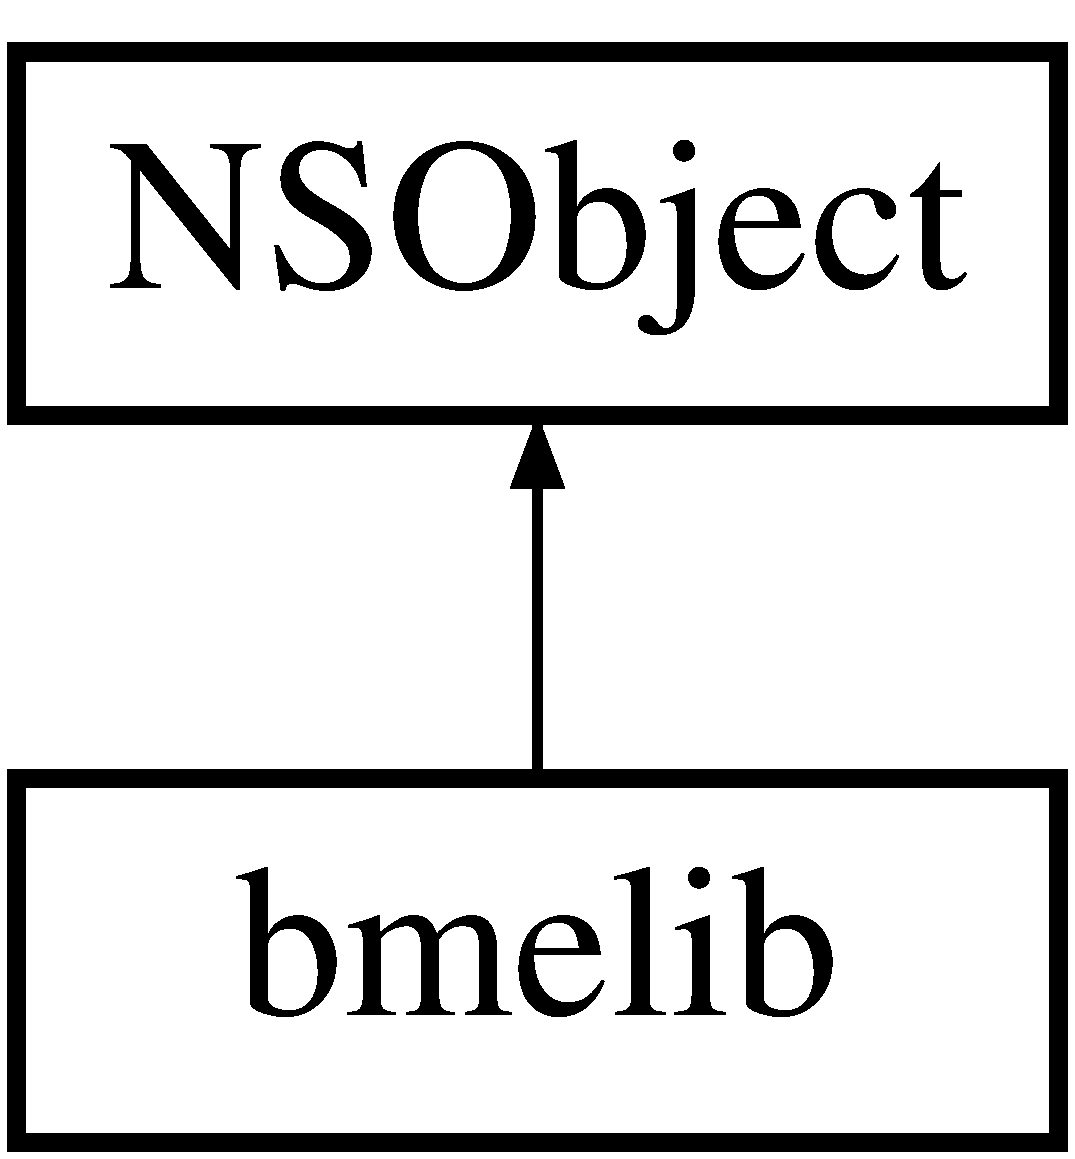
\includegraphics[height=2.000000cm]{interfacebmelib}
\end{center}
\end{figure}
\subsection*{Class Methods}
\begin{DoxyCompactItemize}
\item 
(N\+S\+Data $\ast$) + \mbox{\hyperlink{interfacebmelib_a65726775961be05028282831d3bc83fb}{beep\+Encode\+:::::::}}
\item 
(N\+S\+Mutable\+Array $\ast$) + \mbox{\hyperlink{interfacebmelib_a43dc77d50438093b591f4bb83ebce82f}{allowed\+Modes}}
\item 
(N\+S\+Mutable\+Array $\ast$) + \mbox{\hyperlink{interfacebmelib_a68104948a0882014d1c3e727b10271ee}{allowed\+Frequencies}}
\end{DoxyCompactItemize}


\subsection{Method Documentation}
\mbox{\Hypertarget{interfacebmelib_a68104948a0882014d1c3e727b10271ee}\label{interfacebmelib_a68104948a0882014d1c3e727b10271ee}} 
\index{bmelib@{bmelib}!allowed\+Frequencies@{allowed\+Frequencies}}
\index{allowed\+Frequencies@{allowed\+Frequencies}!bmelib@{bmelib}}
\subsubsection{\texorpdfstring{allowed\+Frequencies()}{allowedFrequencies()}}
{\footnotesize\ttfamily + (N\+S\+Mutable\+Array $\ast$) allowed\+Frequencies \begin{DoxyParamCaption}{ }\end{DoxyParamCaption}}

+(N\+S\+Mutable\+Array $\ast$)allowed\+Frequencies; \mbox{\Hypertarget{interfacebmelib_a43dc77d50438093b591f4bb83ebce82f}\label{interfacebmelib_a43dc77d50438093b591f4bb83ebce82f}} 
\index{bmelib@{bmelib}!allowed\+Modes@{allowed\+Modes}}
\index{allowed\+Modes@{allowed\+Modes}!bmelib@{bmelib}}
\subsubsection{\texorpdfstring{allowed\+Modes()}{allowedModes()}}
{\footnotesize\ttfamily + (N\+S\+Mutable\+Array$\ast$) allowed\+Modes \begin{DoxyParamCaption}{ }\end{DoxyParamCaption}}

+(N\+S\+Mutable\+Array$\ast$)allowed\+Modes; \mbox{\Hypertarget{interfacebmelib_a65726775961be05028282831d3bc83fb}\label{interfacebmelib_a65726775961be05028282831d3bc83fb}} 
\index{bmelib@{bmelib}!beep\+Encode\+:::::::@{beep\+Encode\+:::::::}}
\index{beep\+Encode\+:::::::@{beep\+Encode\+:::::::}!bmelib@{bmelib}}
\subsubsection{\texorpdfstring{beep\+Encode\+:::::::()}{beepEncode:::::::()}}
{\footnotesize\ttfamily + (N\+S\+Data$\ast$) beep\+Encode\+: \begin{DoxyParamCaption}\item[{(N\+S\+String $\ast$)}]{Frequency }\item[{:(float)}]{silence\+Length }\item[{:(float)}]{repetitions }\item[{:(N\+S\+Integer)}]{A\+AC }\item[{:(N\+S\+String $\ast$)}]{gain }\item[{:(float)}]{error }\item[{:(N\+S\+String $\ast$$\ast$)}]{err }\end{DoxyParamCaption}}

+(N\+S\+Data$\ast$)beep\+Encode\+:(\+N\+S\+String$\ast$) mode Frequency \+:(float)frequency silence\+Length \+:(float)sil repetitions \+:(N\+S\+Integer)rep A\+AC \+:(N\+S\+String $\ast$)A\+AC gain \+:(float)gain error \+:(N\+S\+String $\ast$$\ast$)err; 

The documentation for this class was generated from the following file\+:\begin{DoxyCompactItemize}
\item 
bmelib.\+h\end{DoxyCompactItemize}

\hypertarget{interface_view_controller}{}\section{View\+Controller Class Reference}
\label{interface_view_controller}\index{View\+Controller@{View\+Controller}}
Inheritance diagram for View\+Controller\+:\begin{figure}[H]
\begin{center}
\leavevmode
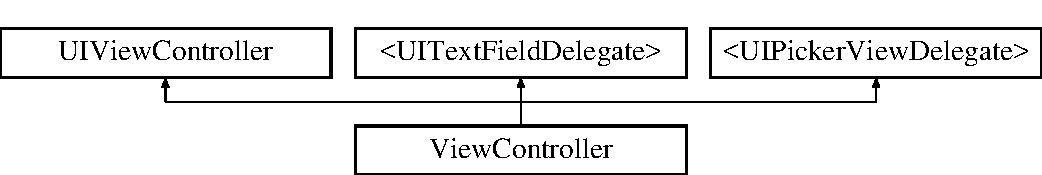
\includegraphics[height=2.000000cm]{interface_view_controller}
\end{center}
\end{figure}
\subsection*{Instance Methods}
\begin{DoxyCompactItemize}
\item 
\mbox{\Hypertarget{interface_view_controller_af998e4b7ee7412df260fe15a1e11593d}\label{interface_view_controller_af998e4b7ee7412df260fe15a1e11593d}} 
(I\+B\+Action) -\/ {\bfseries background\+Button\+Pressed\+:}
\item 
\mbox{\Hypertarget{interface_view_controller_a57c529b23f754b32680910bd113a58d2}\label{interface_view_controller_a57c529b23f754b32680910bd113a58d2}} 
(I\+B\+Action) -\/ {\bfseries slider\+Value\+Changed\+:}
\item 
\mbox{\Hypertarget{interface_view_controller_a04e6382d0883a311916ddf1f96598be5}\label{interface_view_controller_a04e6382d0883a311916ddf1f96598be5}} 
(I\+B\+Action) -\/ {\bfseries go\+Button\+Pressed\+:}
\item 
\mbox{\Hypertarget{interface_view_controller_adfd81c87a0224757b4490cffb7d949af}\label{interface_view_controller_adfd81c87a0224757b4490cffb7d949af}} 
(void) -\/ {\bfseries show\+Picker\+:}
\item 
\mbox{\Hypertarget{interface_view_controller_a5a5e8318b7fbb459130b7a9ca2d8566c}\label{interface_view_controller_a5a5e8318b7fbb459130b7a9ca2d8566c}} 
(void) -\/ {\bfseries hide\+Picker\+:}
\item 
\mbox{\Hypertarget{interface_view_controller_ae930222418ea719390c084f981e010e8}\label{interface_view_controller_ae930222418ea719390c084f981e010e8}} 
(N\+S\+Integer) -\/ {\bfseries selected\+Row\+In\+Picker\+:}
\item 
\mbox{\Hypertarget{interface_view_controller_a05fc90a938185afb08bb8f6b2eb47c20}\label{interface_view_controller_a05fc90a938185afb08bb8f6b2eb47c20}} 
(N\+S\+Mutable\+Data $\ast$) -\/ {\bfseries prepareforplay\+:}
\end{DoxyCompactItemize}
\subsection*{Protected Attributes}
\begin{DoxyCompactItemize}
\item 
\mbox{\Hypertarget{interface_view_controller_a8d82cf652c7d946452f768aa0e945969}\label{interface_view_controller_a8d82cf652c7d946452f768aa0e945969}} 
N\+S\+String $\ast$ {\bfseries mode}
\item 
\mbox{\Hypertarget{interface_view_controller_a219cee1982ff17b000364b551dacd387}\label{interface_view_controller_a219cee1982ff17b000364b551dacd387}} 
N\+S\+String $\ast$ {\bfseries code\+Value1}
\item 
\mbox{\Hypertarget{interface_view_controller_a1e3cc2a7b4071b1f350e3690f74c3761}\label{interface_view_controller_a1e3cc2a7b4071b1f350e3690f74c3761}} 
N\+S\+String $\ast$ {\bfseries code\+Repetition}
\item 
\mbox{\Hypertarget{interface_view_controller_a3db9823387ce30e560710ae927e727a0}\label{interface_view_controller_a3db9823387ce30e560710ae927e727a0}} 
float {\bfseries frequency}
\item 
\mbox{\Hypertarget{interface_view_controller_a40ba6f274aaa3c91ef331b19b5a3e584}\label{interface_view_controller_a40ba6f274aaa3c91ef331b19b5a3e584}} 
float {\bfseries silence\+Length}
\item 
\mbox{\Hypertarget{interface_view_controller_ac0885d91c46e2bdb7aaeb7b129519395}\label{interface_view_controller_ac0885d91c46e2bdb7aaeb7b129519395}} 
float {\bfseries beep\+Mark\+Volume}
\item 
\mbox{\Hypertarget{interface_view_controller_a7249af94e5a016d939f9c914e54600ed}\label{interface_view_controller_a7249af94e5a016d939f9c914e54600ed}} 
float {\bfseries speaker\+Volume}
\item 
\mbox{\Hypertarget{interface_view_controller_ab252479e68a05a57b91f425d537d0996}\label{interface_view_controller_ab252479e68a05a57b91f425d537d0996}} 
int {\bfseries repetitions}
\item 
\mbox{\Hypertarget{interface_view_controller_a347b431066ed1be7814f92d0e1323027}\label{interface_view_controller_a347b431066ed1be7814f92d0e1323027}} 
float {\bfseries gain}
\item 
\mbox{\Hypertarget{interface_view_controller_a232d01fb8b9895b15fe25a3e2852d947}\label{interface_view_controller_a232d01fb8b9895b15fe25a3e2852d947}} 
N\+S\+String $\ast$ {\bfseries A\+AC}
\item 
\mbox{\Hypertarget{interface_view_controller_a42cfeb6de42d8a8da48323379597e962}\label{interface_view_controller_a42cfeb6de42d8a8da48323379597e962}} 
B\+O\+OL {\bfseries is\+Frequency\+Picker\+Open}
\item 
\mbox{\Hypertarget{interface_view_controller_abaa46dd3e6661071d42300268823610f}\label{interface_view_controller_abaa46dd3e6661071d42300268823610f}} 
B\+O\+OL {\bfseries is\+Num\+Of\+Phases\+Picker\+Open}
\item 
\mbox{\Hypertarget{interface_view_controller_a67d1a179e31c834c65065c5873c22aeb}\label{interface_view_controller_a67d1a179e31c834c65065c5873c22aeb}} 
B\+O\+OL {\bfseries ism\+Modes\+Picker}
\item 
\mbox{\Hypertarget{interface_view_controller_a182538813c856b59addf06e8771c5dd0}\label{interface_view_controller_a182538813c856b59addf06e8771c5dd0}} 
N\+S\+Integer {\bfseries scroll\+View\+Offset}
\item 
\mbox{\Hypertarget{interface_view_controller_a84392327e23baf613b3ff12975e3c487}\label{interface_view_controller_a84392327e23baf613b3ff12975e3c487}} 
U\+I\+Text\+Field $\ast$ {\bfseries selected\+Text\+Field}
\end{DoxyCompactItemize}
\subsection*{Properties}
\begin{DoxyCompactItemize}
\item 
\mbox{\Hypertarget{interface_view_controller_a658045907f0a46585f030bd3917647aa}\label{interface_view_controller_a658045907f0a46585f030bd3917647aa}} 
I\+B\+Outlet U\+I\+Button $\ast$ {\bfseries background\+Button}
\item 
\mbox{\Hypertarget{interface_view_controller_ab5cab3313406bf6a8df75069d7882f83}\label{interface_view_controller_ab5cab3313406bf6a8df75069d7882f83}} 
I\+B\+Outlet U\+I\+Scroll\+View $\ast$ {\bfseries scroll\+View}
\item 
\mbox{\Hypertarget{interface_view_controller_aa7241ff6148bdd575c52562c478bbb3a}\label{interface_view_controller_aa7241ff6148bdd575c52562c478bbb3a}} 
I\+B\+Outlet U\+I\+Picker\+View $\ast$ {\bfseries m\+Modes\+Picker}
\item 
\mbox{\Hypertarget{interface_view_controller_a7401ac0ce86a2e7fddde9670289fb464}\label{interface_view_controller_a7401ac0ce86a2e7fddde9670289fb464}} 
I\+B\+Outlet U\+I\+Picker\+View $\ast$ {\bfseries picker\+View\+Frequency}
\item 
\mbox{\Hypertarget{interface_view_controller_acaca00ae6443167be2e39fb354d994d1}\label{interface_view_controller_acaca00ae6443167be2e39fb354d994d1}} 
I\+B\+Outlet U\+I\+Slider $\ast$ {\bfseries slider\+Speaker\+Volume}
\item 
\mbox{\Hypertarget{interface_view_controller_a3235938877df5d68815d024b4fe21dda}\label{interface_view_controller_a3235938877df5d68815d024b4fe21dda}} 
I\+B\+Outlet U\+I\+Text\+Field $\ast$ {\bfseries text\+Field\+Frequency}
\item 
\mbox{\Hypertarget{interface_view_controller_a8f1578901abd9346b8efb773d98c8e49}\label{interface_view_controller_a8f1578901abd9346b8efb773d98c8e49}} 
I\+B\+Outlet U\+I\+Text\+Field $\ast$ {\bfseries text\+Field\+Silence\+Length}
\item 
\mbox{\Hypertarget{interface_view_controller_a6dee8135217f36768cebea5a811d8d8d}\label{interface_view_controller_a6dee8135217f36768cebea5a811d8d8d}} 
I\+B\+Outlet U\+I\+Text\+Field $\ast$ {\bfseries text\+Field\+Code\+Value1}
\item 
\mbox{\Hypertarget{interface_view_controller_a080747fe7745595bb7ae2eb7d12e4b0a}\label{interface_view_controller_a080747fe7745595bb7ae2eb7d12e4b0a}} 
I\+B\+Outlet U\+I\+Text\+Field $\ast$ {\bfseries text\+Field\+Repetitions}
\item 
\mbox{\Hypertarget{interface_view_controller_a4b23b290032fb1c804c327a60494c129}\label{interface_view_controller_a4b23b290032fb1c804c327a60494c129}} 
I\+B\+Outlet U\+I\+Text\+Field $\ast$ {\bfseries text\+Field\+Beep\+Mark\+Volume}
\item 
\mbox{\Hypertarget{interface_view_controller_aae24f60d8ca8184fd18aad8785f4d5ad}\label{interface_view_controller_aae24f60d8ca8184fd18aad8785f4d5ad}} 
I\+B\+Outlet U\+I\+Text\+Field $\ast$ {\bfseries text\+Field\+Mode}
\end{DoxyCompactItemize}


The documentation for this class was generated from the following files\+:\begin{DoxyCompactItemize}
\item 
View\+Controller.\+h\item 
View\+Controller.\+mm\end{DoxyCompactItemize}

\hypertarget{category_view_controller_07_08}{}\section{View\+Controller() Category Reference}
\label{category_view_controller_07_08}\index{View\+Controller()@{View\+Controller()}}
\subsection*{Properties}
\begin{DoxyCompactItemize}
\item 
\mbox{\Hypertarget{category_view_controller_07_08_ad20cdcf7e661043a57407748b371f214}\label{category_view_controller_07_08_ad20cdcf7e661043a57407748b371f214}} 
A\+V\+Audio\+Player $\ast$ {\bfseries player}
\end{DoxyCompactItemize}


The documentation for this category was generated from the following file\+:\begin{DoxyCompactItemize}
\item 
View\+Controller.\+mm\end{DoxyCompactItemize}

%--- End generated contents ---

% Index
\backmatter
\newpage
\phantomsection
\clearemptydoublepage
\addcontentsline{toc}{chapter}{Index}
\printindex

\end{document}
